This chapter introduces the theoretical fundamentals underlying this research. Although these concepts will be presented with an introductory approach, a basic understanding of Machine Learning and Neural Networks is expected. However, this section will cover Musical Computation, FM Synthesis, Fourier Transform, Neural Networks, and One Dimensional Convolutional Neural Networks.

\section{Musical Computation}

Musical computation is a broad and interdisciplinary field that encompasses all aspects of musical processing through a computer. It is beyond the scope of this thesis to provide a comprehensive overview of this field; however, for the purposes of this study, it is important to cover the basic elements of sound and the fundamentals of audio digitization.

\subsection{Sound elements}

Audio is a mechanical compression wave that travels through the air. This type of wave can be converted into an electrical signal through microphones, which consist of an arrangement of coils and magnets. As a wave, its main elements are:

\begin{itemize}
\item Pitch: The fundamental frequency of a sound, which determines whether it is low or high. The higher the frequency, the higher the pitch.
\item Duration: The length of time a sound is sustained and can be heard.
\item Loudness (or amplitude): The intensity or energy level of a sound. In terms of a wave, it corresponds to the amplitude of the sound wave.
\item Timbre: Like the color of a visual object, timbre refers to the quality or "color" of a sound. This aspect will be treated in more detail in the next section.
\end{itemize}

It is important to highlight that although sound can be described in terms of the aspects mentioned above, hearing is mainly a cognitive process. Therefore, sound comparison cannot be fully addressed by mathematical tools, leaving a significant space for perceptual comparison and classification (not to mention aspects related to personal preferences).

\subsubsection{Sound timbre}

Another important aspect of acoustic sounds is timbre, which can be understood as the “color of sound.”

From a mathematical point of view, timbre varies according to the harmonics present in a sound sample, or, in other words, according to the set of oscillations that compose the sound.

In the case of acoustic instruments, what happens is that the air vibrations produced by the instrument are not simple pure sinusoids. In fact, when a string vibrates, or when air resonates inside a tube, many parts of the instrument's body vibrate simultaneously, and the frequency with which each part vibrates differs according to its composition, position, and other factors. The result is that each instrument has a unique sound, especially in the case of handcrafted wooden instruments such as violins or cellos.

To obtain a clear visualization of this aspect, it is common to convert a sound sample from the time domain to the frequency domain using a Fourier Transform technique.

For example, consider the image~\ref{fig:time_domain_violin} which presents violin audio sample in time domain, and the image \ref{fig:frequency_domain_violin} which presents the same audio, but in frequency domains.

\begin{figure}[h]
    \centering
    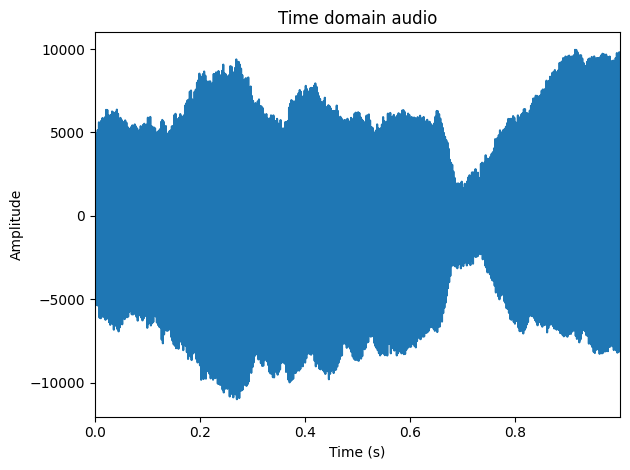
\includegraphics[width=\linewidth]{../images/time_domain_violin.png}
    \caption{One second time domain violin sample.}
    \label{fig:time_domain_violin}
\end{figure}

\begin{figure}[h]
    \centering
    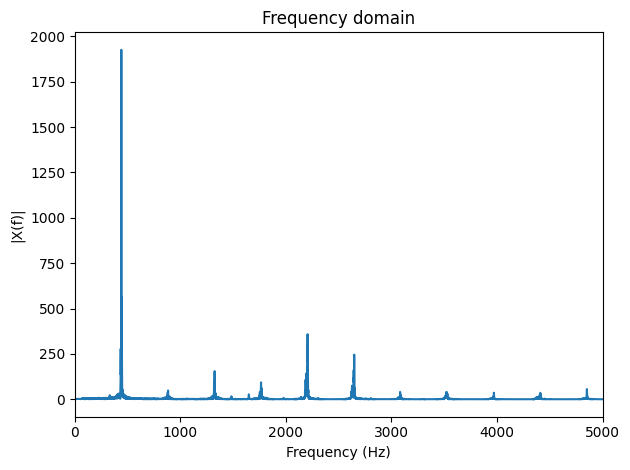
\includegraphics[width=\linewidth]{../images/frequency_domain_violin.png}
    \caption{The same one second frequency domain violin sample.}
    \label{fig:frequency_domain_violin}
\end{figure}

As the figures show, there is a main frequency that defines the pitch of the sound, along with many other frequencies that allow the ear to identify the instrument and distinguish between different kinds of sounds.

\subsection{Audio digitalization}

A microphone converts a pressure wave into an electrical waveform. However, in computational music, the audio signal must be discretized to be represented as a digital audio file. The primary process for digital audio representation is sampling.

Sampling consists of recording a sequence of wave amplitudes at fixed intervals. For example, if a sound is recorded using a sampling rate of 22,100 Hz, it means that the computer will capture 22,100 audio samples per second.

\begin{figure}[htb]
 \caption{Signal sampling}
 \label{fig:signal_sampling}
 \centering
 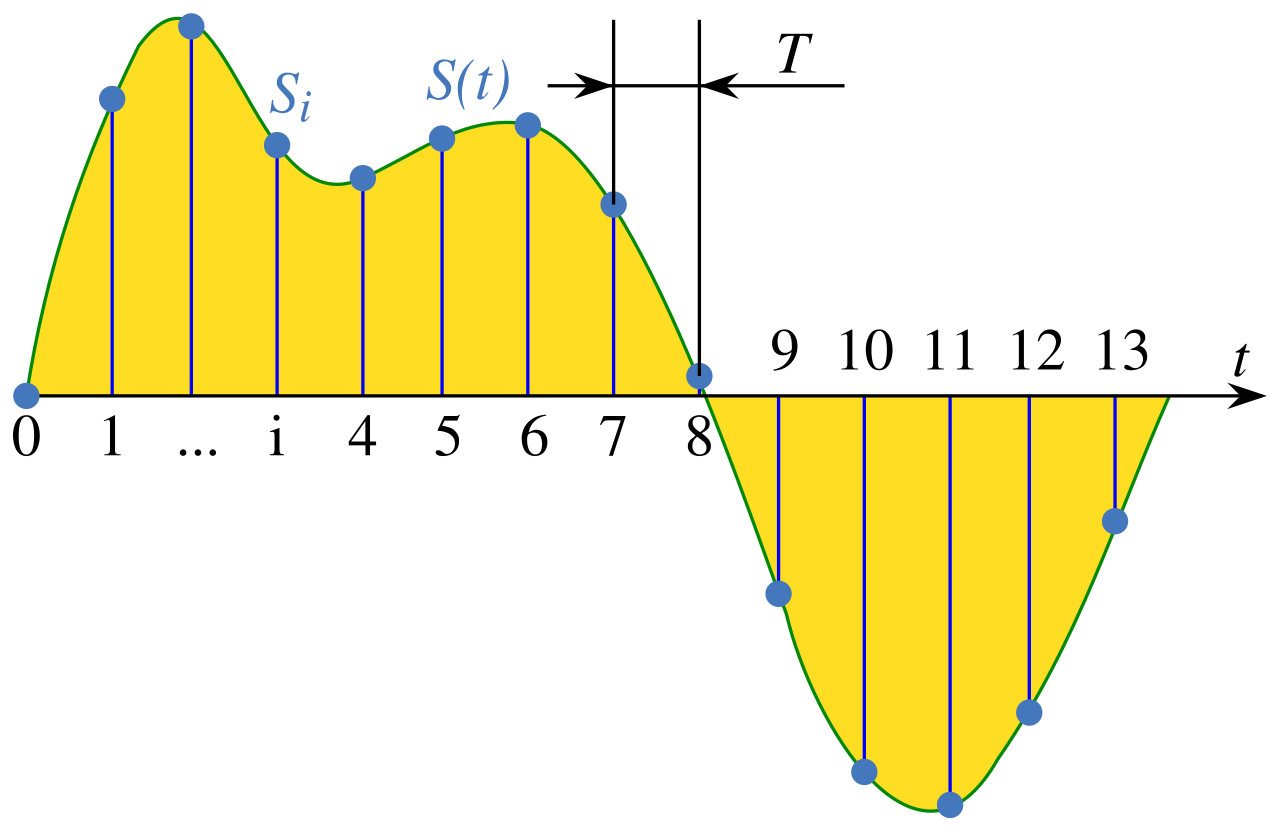
\includegraphics[scale=0.2]{images/signal_sampling.png}
 \fdireta{usp:logo}
\end{figure}

This approach is very efficient because human hearing can detect frequencies between 20 Hz and 20,000 Hz. However, for most musical sounds, the maximum frequency is typically below 10 kHz (in fact, even a violin—one of the highest-pitched instruments—reaches only around 3,500 Hz). And according to the Nyquist-Shannon Theorem, to properly sample a periodic signal, the sampling rate must be at least twice the frequency of the highest component of the signal.

Thus, 22,100 Hz can be a good sampling rate for recording music while saving disk space. However, if the goal is to cover the full range of human hearing, higher rates, such as 44,200 Hz, can also be used.

Note that with this process, all sound elements highlighted before, can be recorded and reprocedure later.

\subsection{Sound synthesis}

After the development of sound recording techniques, musical computation evolved toward the creation of artificial waveforms. Of course, before digital audio synthesis, there were several techniques that allowed analog synthesis. However, the underlying idea is essentially quite similar.

In summary, audio synthesis techniques can be divided into three basic types:

\begin{itemize}
\item \textbf{Additive synthesis:} Perhaps the most straightforward idea from a mathematical point of view. It consists of generating each frequency component of a desired timbre separately and then summing them. In fact, it is more like a weighted sum, since each component is weighted according to its contribution to the timbre. A normalization step is commonly applied after the process to avoid amplitude overload.

\item \textbf{Subtractive synthesis:} The opposite of the previous technique, but historically more common due to its effectivenessa and lower cost. In short, it consists of taking a complex waveform, rich in harmonics, and applying various filters to obtain the desired sound. It is more empirical than additive synthesis (which is based on spectral analysis), but simpler to implement and less computationally intensive. Typically, the original waveforms are complex ones such as the sawtooth wave, square wave, or triangular wave.

\item \textbf{FM synthesis:} Another empirical approach to sound synthesis, which will be addressed in detail in a later section. In short, it consists of altering a simple waveform by applying a high-frequency modulation, not to the generated waveform itself, but directly to the frequency parameter of the carrier oscillator. This kind of distortion of the base frequency produces mirrored harmonics that enrich the timbre of the sound. It is up to the musician to choose the appropriate parameters to produce the desired timbre.
\end{itemize}

There are many other techniques that could be mentioned; however, these three represent the most direct forms of synthesis, or the most purely mathematical ones, in the sense that they do not require manipulation of pre-recorded audio.

\subsubsection{ADSR Audio envelop}

Another important technique for achieving good results is the so-called “Attack, Decay, Sustain, and Release (ADSR) envelope”, which consists of applying a multiplicative function to the waveform, altering only its amplitude.

The basic idea is to control the sound intensity by simulating the natural behavior of acoustic sounds. Typically, an ADSR envelope is defined as a function with a domain between 0 and 1, which is applied to the generated waveform:

\begin{figure}[h]
    \centering
    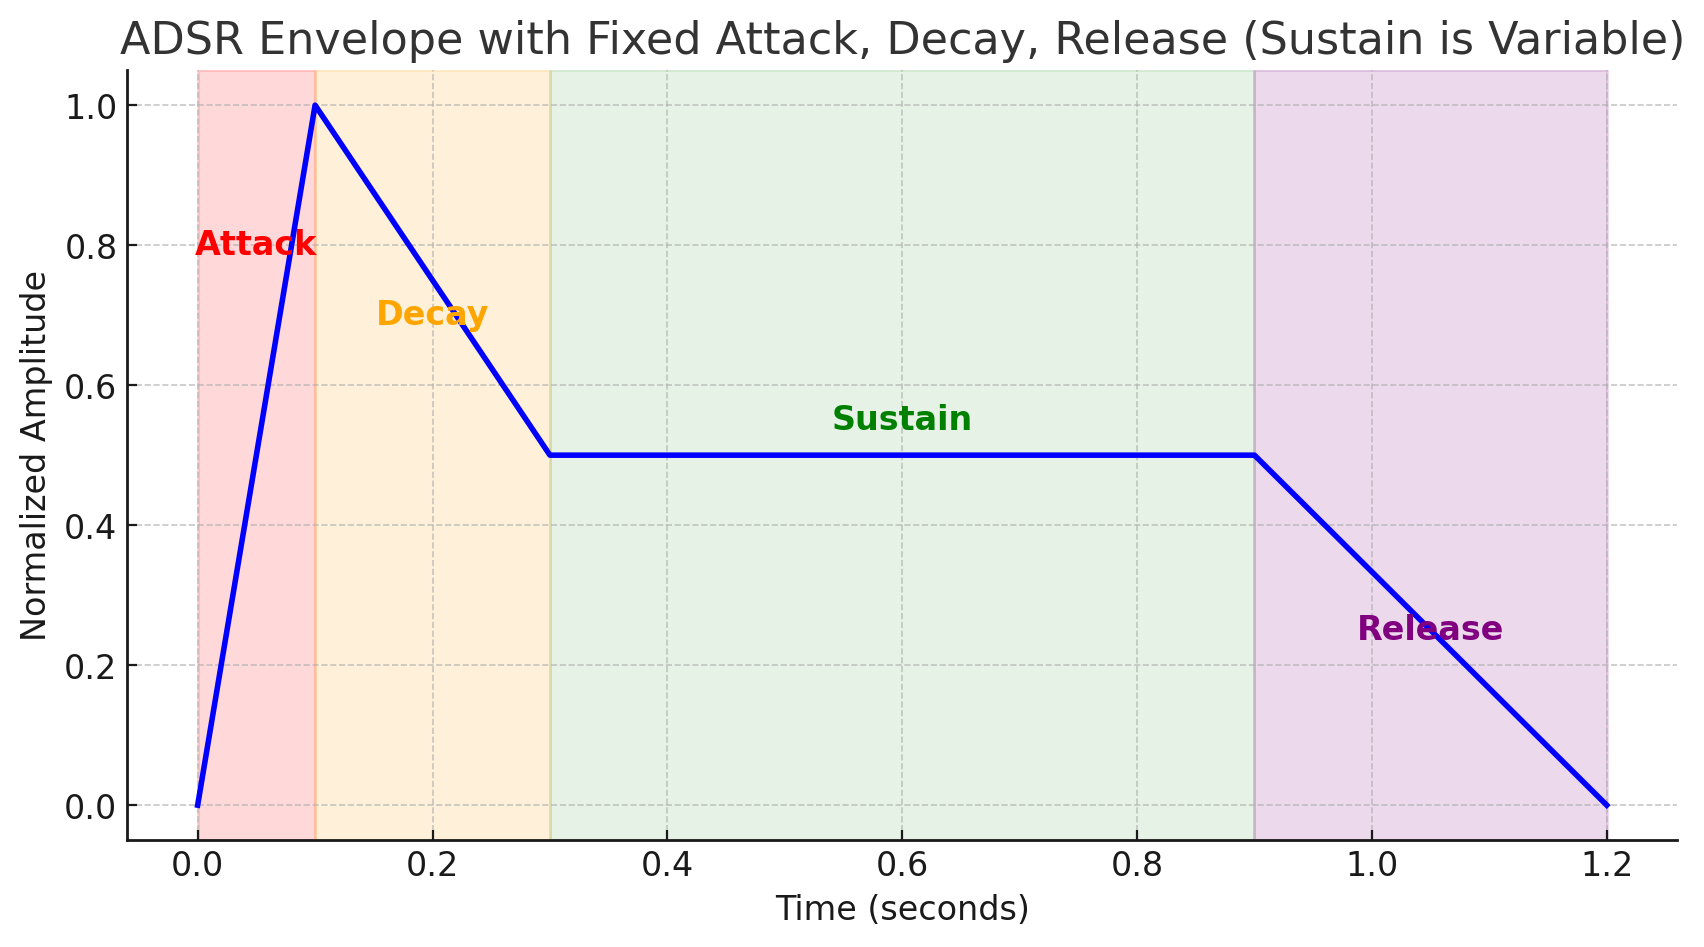
\includegraphics[width=\linewidth]{../images/adsr.png}
    \caption{ADSR linear envelop.}
    \label{fig:adsr_linear_envelop}
\end{figure}

The ADSR envelope can be understood as an amplitude function:

\[
y(t) = e(t) \cdot s(t)
\]

Where:

\begin{itemize}
\item \( s(t) \): the raw generated sound wave.
\item \( e(t) \): the ADSR envelope function (normalized amplitude ranging from 0 to 1).
\item \( y(t) \): the resulting sound.
\end{itemize}

Although real audio samples can show a wide variation of envelope behaviors, it is common practice to use a linear function to achieve the goal, since the human ear is more sensitive to abrupt changes and to relative differences. However, for long time variations, the ear can still perceive the change, which is why some synthesizers allow the use of exponential or logarithmic functions as well.

\subsection{FM Synthesis}

As shown in the previous sections, one of the most popular sound synthesis techniques is Frequency Modulation Synthesis (FM Synthesis), which was introduced by John M. Chowning in his famous paper “The Synthesis of Complex Audio Spectra by Means of Frequency Modulation”, published at the Stanford Artificial Intelligence Laboratory.

Chowning explored the effects of frequency modulation when applied with high frequencies, close to the audible range, instead of the traditional use of inaudible frequencies.

In fact, the concept of frequency modulation was already well known before this paper; however, it had been used mainly in radio transmission of music or to apply slight distortions through low-frequency oscillators (LFOs), producing effects such as vibrato.

As Chowning himself pointed out in his paper, when the technique is applied to vary the frequency of the carrier wave through a high-frequency modulator wave, it “results in a surprising control of audio spectra” (\cite{chowning1973synthesis}).

In summary, considering only two oscillators: the main one, called the carrier, and the modulator, so the instantaneous frequency of the output audio can be expressed by the following function:

\[
f(t) = f_c + I \cdot \sin(2\pi f_m t)
\]

Where:

\begin{itemize}
\item \( f(t) \): the instantaneous frequency of the generated sound wave.
\item \( f_c \): the original frequency of the carrier wave.
\item \( I \): the modulation index, which defines the intensity of the modulation (the greater the value, the more harmonics are generated).
\item \( f_m \): the frequency of the modulator wave (which determines the spacing of the harmonics).
\item \( t \): the time variable.
\end{itemize}

The most important point, however, is that this simple manipulation results in symmetric sidebands around the carrier frequency, spaced at multiples of \( f_m \).

For a more intuitive understanding, if a carrier frequency \( f_m \) is modulated by a frequency \( f_m \), the resulting spectrum will contain:

\[
f_c \pm n f_m
\]

For example, by choosing \( f_c = 440 \) and \( f_m = 220 \), the resulting wave will contain frequency components such as 220 Hz, 440 Hz, 660 Hz, 880 Hz, and so on, with decreasing amplitudes (the amplitudes follow the Bessel coefficients, but this discussion is beyond the scope of this article).

The last important characteristic of Frequency Modulation Synthesis concerns the ratio between the carrier frequency and the modulator frequency \( f_c / f_m \), since this ratio directly influences the perceived audio result.

This ratio determines whether the generated harmonics align with the natural harmonic series (widely used by musicians) or not:

\begin{itemize}
    \item If the ratio is an integer number, the harmonic sidebands (in the spectral view) will appear as integer multiples of \( f_c \), generating harmonic sounds similar to those of real instruments (consistent with traditional music theory).
    \item If the ratio is not an integer value, the harmonic sidebands will not align perfectly with \( f_c \), and the generated sound may appear metallic or dissonant (but, this effect is useful for creating sounds such as bells or for producing special audio effects).
\end{itemize}

\subsection{Audio comparison}

The task of audio comparison is not straightforward, especially when the goal is to achieve equality in terms of human perception. It can be complex, computationally demanding, and inherently subjective.

However, as described in the section on timbre, one intuitive and efficient way to approach this problem is by comparing the audio in its spectral representation, since timbre is precisely defined by this combination of frequencies.

That said, this approach alone is not sufficient, because the Fourier Transform considers the entire audio signal at once, mixing different parts of a sound sample. For example, if a sample contains three different pitches in sequence, its frequency-domain representation will show them simultaneously, which may give the impression that the timbre is a mixture of all these pitches (similar to a chord rather than a sequence).

In fact, according to \cite{claesson2021resynthesis}, FFT-based spectral comparison is valid but only a part of the solution. He highlights the following metrics:

\begin{itemize}
    \item \textbf{FFT Distance:} This metric consists of computing the Fast Fourier Transform (FFT) of the two samples being compared and then calculating the Euclidean distance between them. The result can be normalized so that the maximum distance is 1 and the minimum is 0.
    \item \textbf{Short Time Fourier Transform (STFT) Distance:} Equivalent to the FFT Distance, but calculated over short, overlapping slices of the sample, which provides time-localized spectral information.
    \item \textbf{Log-Mel Spectogram Distance:} Similar to the previous metrics, but based on the Log-Mel Spectrogram, which is essentially an adaptation of the FFT spectrum that incorporates human auditory perception. In summary, the Log-Mel Spectrogram is obtained by computing the STFT, mapping the frequencies onto the Mel scale (explained later in this document), and finally projecting the amplitudes onto a logarithmic scale.
\end{itemize}

In addition to these three metrics, \cite{claesson2021resynthesis} also recommends the use of Euclidean Distance of the Envelope to compare audio envelopes. This approach can be very useful, but since this work is focused on the similarity between original and synthesized audio in terms of timbre, the envelope comparison, while important for real-world applications, falls outside the scope of the present study.

\subsubsection{Mel-Scale Representation}

The Mel scale was proposed by Stevens, Volkmann, and Newman in 1937 (\cite{claesson2021resynthesis}), and its main purpose is to reflect the human perception of frequency.

The key difference from the linear scale is that, as the values on the scale increase, the perceptual difference between two adjacent points becomes smaller.

In fact, the Mel scale maps linear frequencies onto a logarithmic scale. A frequency \( f \) s converted to the Mel scale through the following formula:

\[
\text{Mel}(f) = 2595 \log_{10} \left( 1 + \frac{f}{700} \right)
\]

For a better understanding of this conversion, consider the following graph, which compares the linear hertz scale with the Mel scale:

\begin{figure}[h]
    \centering
    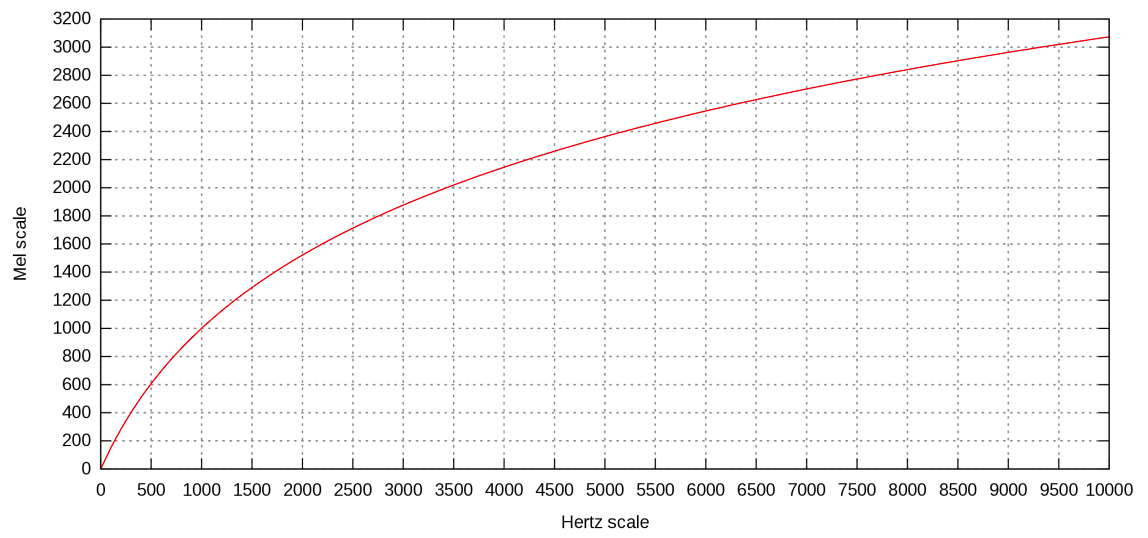
\includegraphics[width=\linewidth]{../images/mel_scale.png}
    \caption{Comparision between linear hertz scale and Mel scale (\cite{claesson2021resynthesis}).}
    \label{fig:mel_scale_comparison}
\end{figure}

It is a very useful metric for audio comparison, as it takes into account the human auditory perception of frequency.

\section{1D Convolutional Neural Networks}

\subsection{History and motivation}

Convolutional Neural Networks (CNNs) originated in the 1990s with the introduction of the "LeNet" model. Since their inception, CNNs have demonstrated remarkable results in classification tasks.

Although this type of neural network went through a period of relative stagnation—due to the rise of alternative machine learning paradigms such as Support Vector Machines and Bayesian Networks—CNNs eventually became the de facto standard for computer vision problems, including object detection, image classification, and other image-based machine learning challenges.

The significant breakthrough in the use of CNNs can be attributed to two main factors: (1) the simplicity with which CNNs handle input data, such as images; and (2) the efficient use of computational resources during training.

Regarding simplicity, since the advent of CNNs, many image-based machine learning tasks no longer require extensive pre-processing before applying learning algorithms to solve the target problem.

For example, consider the problem of bird species classification based on images. In such a task, it is easy to observe that for many species, simple color patterns (e.g., on the bird's plumage) may be sufficient for identification. For other species, the analysis of connected components in the image—such as textures and visual patterns—can play a crucial role. Furthermore, in other cases, the frequency of color variations across the image may serve as a key classification feature.

Therefore, different filters are required to detect distinct properties in the images, making it possible to apply machine learning techniques—such as decision trees—for effective image classification.

In addition, several other important factors must be considered to improve classification performance, including image rotation, scale variation, translation, lighting conditions, and more.
